\section{Introduction}
\label{vlprompt:sec:introduction}

Building on Chapter~3, this chapter addresses a second obstacle to learning relational structure: rare and ambiguous relations are often difficult to resolve from visual evidence alone.
The setting remains closed-set PSG, but the model now incorporates language-derived relational knowledge. Under the argument in Section~\ref{sec:unifying_argument}, access to this knowledge is insufficient unless it is aligned with the relevant object pair and grounded in visual evidence. This chapter therefore learns when and how language features should inform relation prediction.

Panoptic scene graph generation (PSG)~\citep{yang2022panoptic} extends scene graph generation (SGG)~\citep{lu2016visual} by incorporating panoptic segmentation~\citep{kirillov2019panoptic} to capture richer and more detailed representations of images, including both ``thing''~\citep{lin2014microsoft} and ``stuff''~\citep{caesar2018coco} object classes.
PSG constructs a directed graph to represent an image, where nodes signify objects and edges capture the relations between objects.
As a bridge between vision and language~\citep{zhu2022scene}, PSG has a multitude of downstream applications such as visual question answering~\citep{hildebrandt2020scene}, image captioning~\citep{gao2018image, chen2020say}, and visual reasoning~\citep{aditya2018image, shi2019explainable}; furthermore, it can also benefit relevant fields like embodied navigation~\citep{singh2023scene} and robotic action planning~\citep{amiri2022reasoning}.

Notwithstanding, the current performance of PSG~\citep{yang2022panoptic, zhou2023hilo, wang2023pair, li2023panoptic, hayder2024dsgg, lorenz2024fair, zhou2025openpsg} remains unsatisfactory, limiting its downstream applications.
The essential reason lies in the severe long-tail problem in relation categories: for instance, in the PSG dataset~\citep{yang2022panoptic}, the top three most frequent relation categories account for over 50\% of entire samples, with numerous rare relations appearing less than 1\%.
PSG models thus struggle to accurately predict these rare relations.

Recent methods~\citep{lyu2022fine, dong2022stacked, li2022ppdl, zhang2022fine, deng2022hierarchical, zhou2023hilo, yu2023visually, hayder2024dsgg, im2024egtr, li2024leveraging, lorenz2024fair} have made progress in addressing the long-tail problem, mainly exploiting the strength of vision information for relation prediction, whilst overlooking the language information in PSG.
The integration of language information is however important to provide additional common sense knowledge for objects and their relations. 
For example, in the two images of Fig.~\ref{vlprompt:fig:motivation}, the relation between the person and the elephant is \textit{cleaning}.
In the image 2 of Fig.~\ref{vlprompt:fig:motivation}, where the person is on the elephant's back \textit{cleaning} it, this scenario can easily lead previous vision-only models to classify the relation as \textit{riding}.
In contrast, our vision-language model can utilize language information like ``a person cleans an elephant using brushes on the back of the elephant'', thus precisely predicting the relation as \textit{cleaning}.

In SGG task, some methods~\citep{he2022towards, dong2022stacked} have recognized the importance of incorporating language information besides vision. 
However, the way language information is utilized in these works is limited to category names of objects or relations, providing no further context and hence not fully addressing the long-tail problem.
The same observation goes to methods like~\citet{gu2019scene, zareian2020bridging}, which integrate knowledge graphs into the SGG task.
With the rapid development of Large Language Models (LLMs)~\citep{chatgpt, touvron2023llama}, acquiring richer language information, instead of merely the concepts of objects or relations, becomes much easier than before.

\begin{figure}[t]
    \centering
    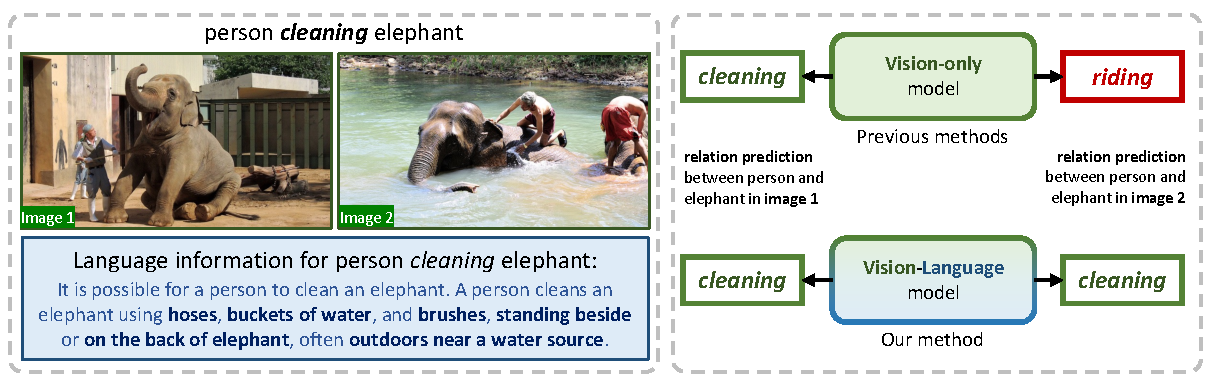
\includegraphics[width=1.0\linewidth]{Chapter4/Figures/motivation_v4.pdf}
    \caption{Comparison between previous PSG methods and ours.
    \textbf{Left}: Images of ``person \textit{cleaning} elephant'' in two different scenes, accompanied by snippets of descriptions about ``person \textit{cleaning} elephant'' obtained from LLMs.
    \textbf{Right}: Previous vision-only models can predict the \textit{cleaning} relation between the person and elephant in image 1, but often classify image 2's relation as \textit{riding} due to the person's position on the back of the elephant.
    Our vision-language model, enriched with language information, precisely identifies the \textit{cleaning} relation in both images.
    }
    \label{vlprompt:fig:motivation}
\end{figure}

This chapter introduces a novel \textbf{V}ision-\textbf{L}anguage \textbf{Prompt}ing (\textbf{VLPrompt}) model, which leverages rich language information from LLMs to help predict relations between objects in visual images.
The language information serves as a powerful supplement to relation prediction, especially for rare ones.
Our model comprises three parts, forming a complete system implementation of our proposed idea.
The first is the \emph{vision feature extractor}, where we process the input image with a panoptic segmentation network adapted from Mask2Former~\citep{cheng2022masked} to extract features of different objects.
We pair and concatenate these object features and integrate their corresponding spatial information to form the vision prompting features.
In contrast, in the second part, the \emph{language feature extractor}, we employ the chain-of-thought technique~\citep{wei2022chain} to design various prompts, aiming to stimulate LLMs to propose context-rich language information for potential relations between a subject-object pair or judge a specific subject-relation-object triplet.
These two functions are realized via the carefully designed relation proposer prompt and relation judger prompt.  
Subsequently, these language descriptions are transformed into language features using a pre-trained text encoder.
Finally, in the third part, the \emph{vision-language prompter}, we design a novel dual attention-based prompter network to facilitate the interaction between vision features and the two complimentary language features respectively, resulting into two sets of relation predictions.
They are combined via a MLP-based gating network to take the strength of both for final relation prediction.
The whole VLPrompt is trained end-to-end.

Extensive experiments on the PSG dataset~\citep{yang2022panoptic} demonstrate that our VLPrompt significantly enhances the PSG performance, especially in predicting rare relations, highlighting the importance of integrating language information from LLMs to support relation prediction in the PSG task.
Within the thesis, VLPrompt forms the second step of the PSG progression: Chapter~3 established a stronger visual baseline for long-tail relation prediction, this chapter adds language-assisted reasoning on top of that closed-set setting, and Chapter~5 then extends the same line to open-set PSG.
